\subsection{Einleitung}

Bei HiL (\acrlong{hil}) handelt es sich um eine Simulation, bei welcher die Sensoren und Aktuatoren des Systems getestet werden sollen. Diese Simulationen werden oft für eingebettet Systeme verwendet. Der Vorteil liegt darin, dass bei einem Modellabsturz keine Schäden entstehen und der Vorgang zu diesem Ereignis klar verfolgbar ist durch die Log Dateien.

\begin{figure}[ht]
	\begin{center}
		\begin{subfigure}{0.49\textwidth}
			\begin{center}
		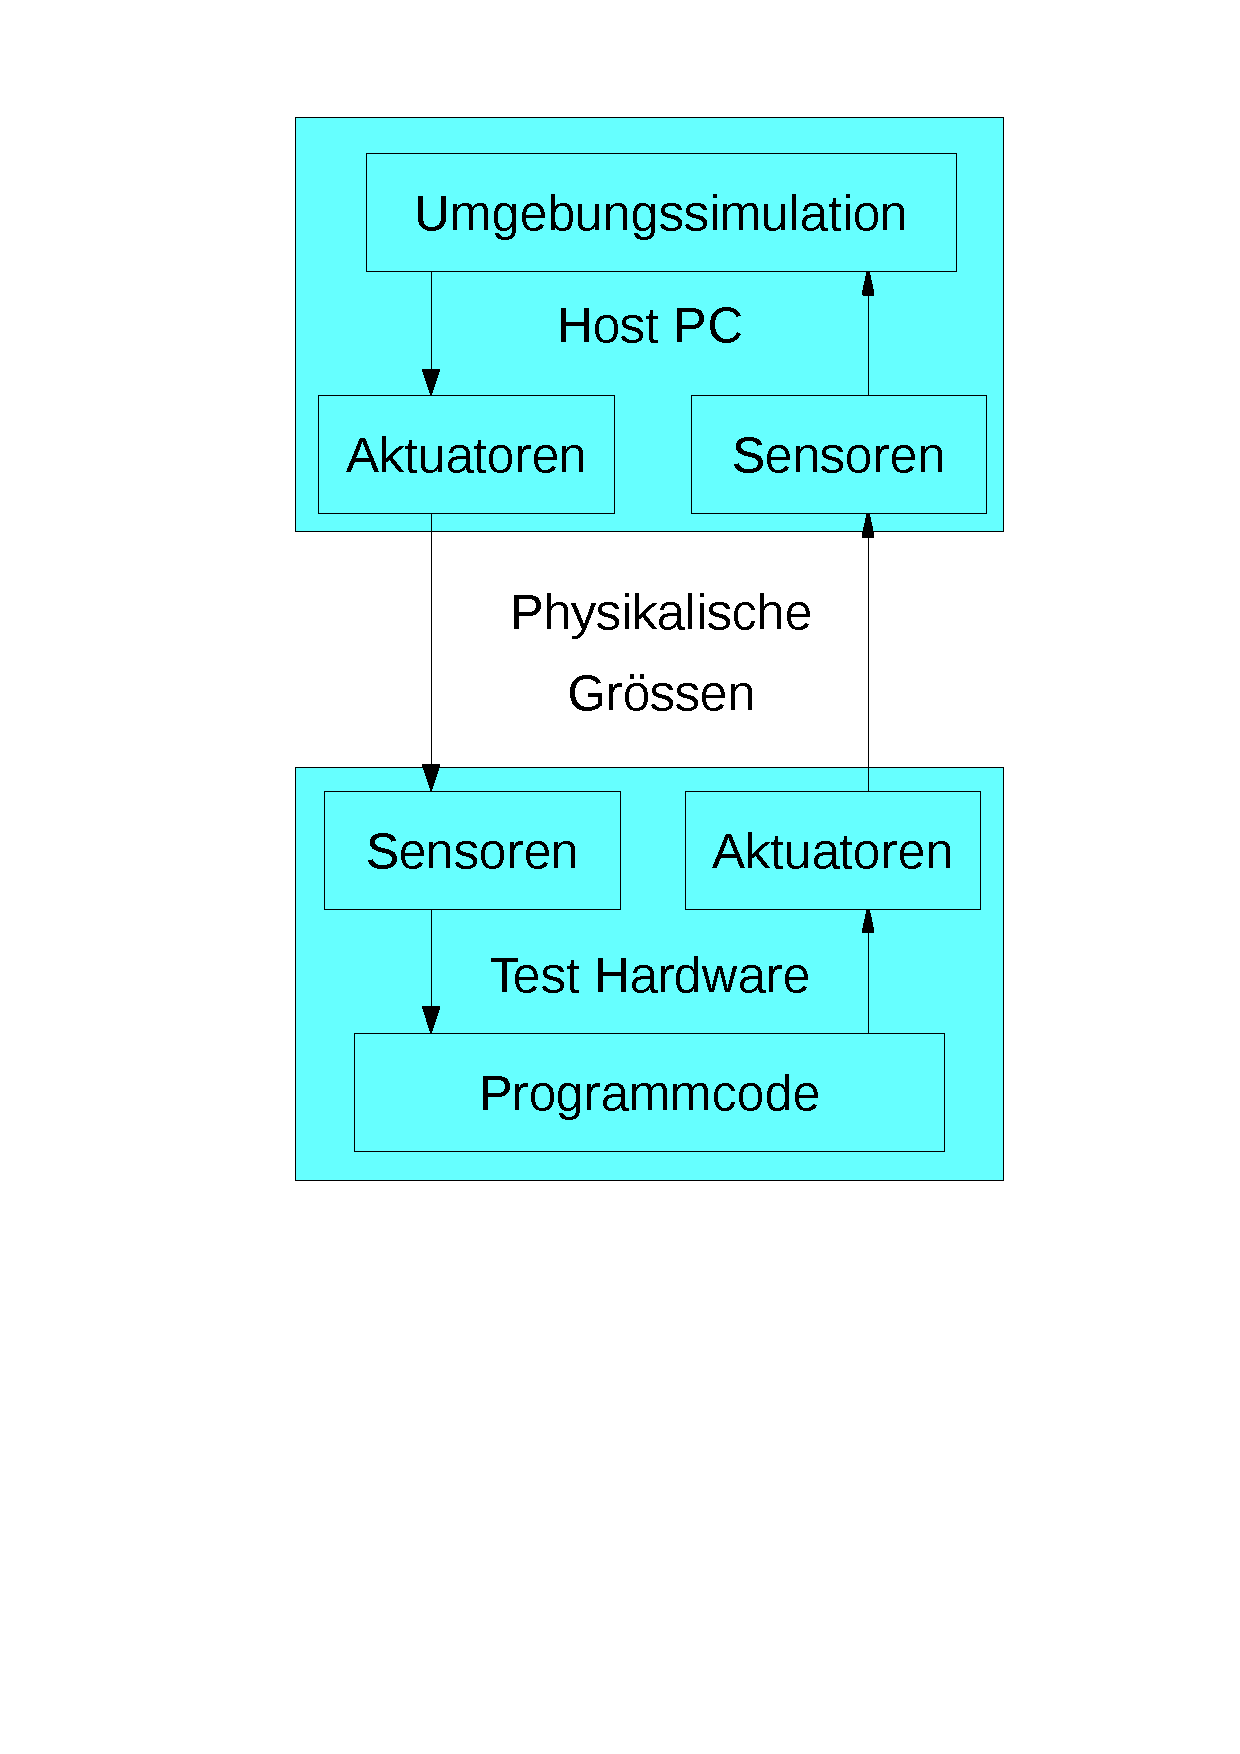
\includegraphics[height=0.33\paperheight, trim={5cm 9.5cm 4cm 2cm},clip]{pic/35_hil/hil_1.pdf} 
		\caption{Allgemeiner Hil Aufbau}
		\label{fig:hil_normal}
		\end{center}
		\end{subfigure}
		\begin{subfigure}{0.49\textwidth}
		\begin{center}
		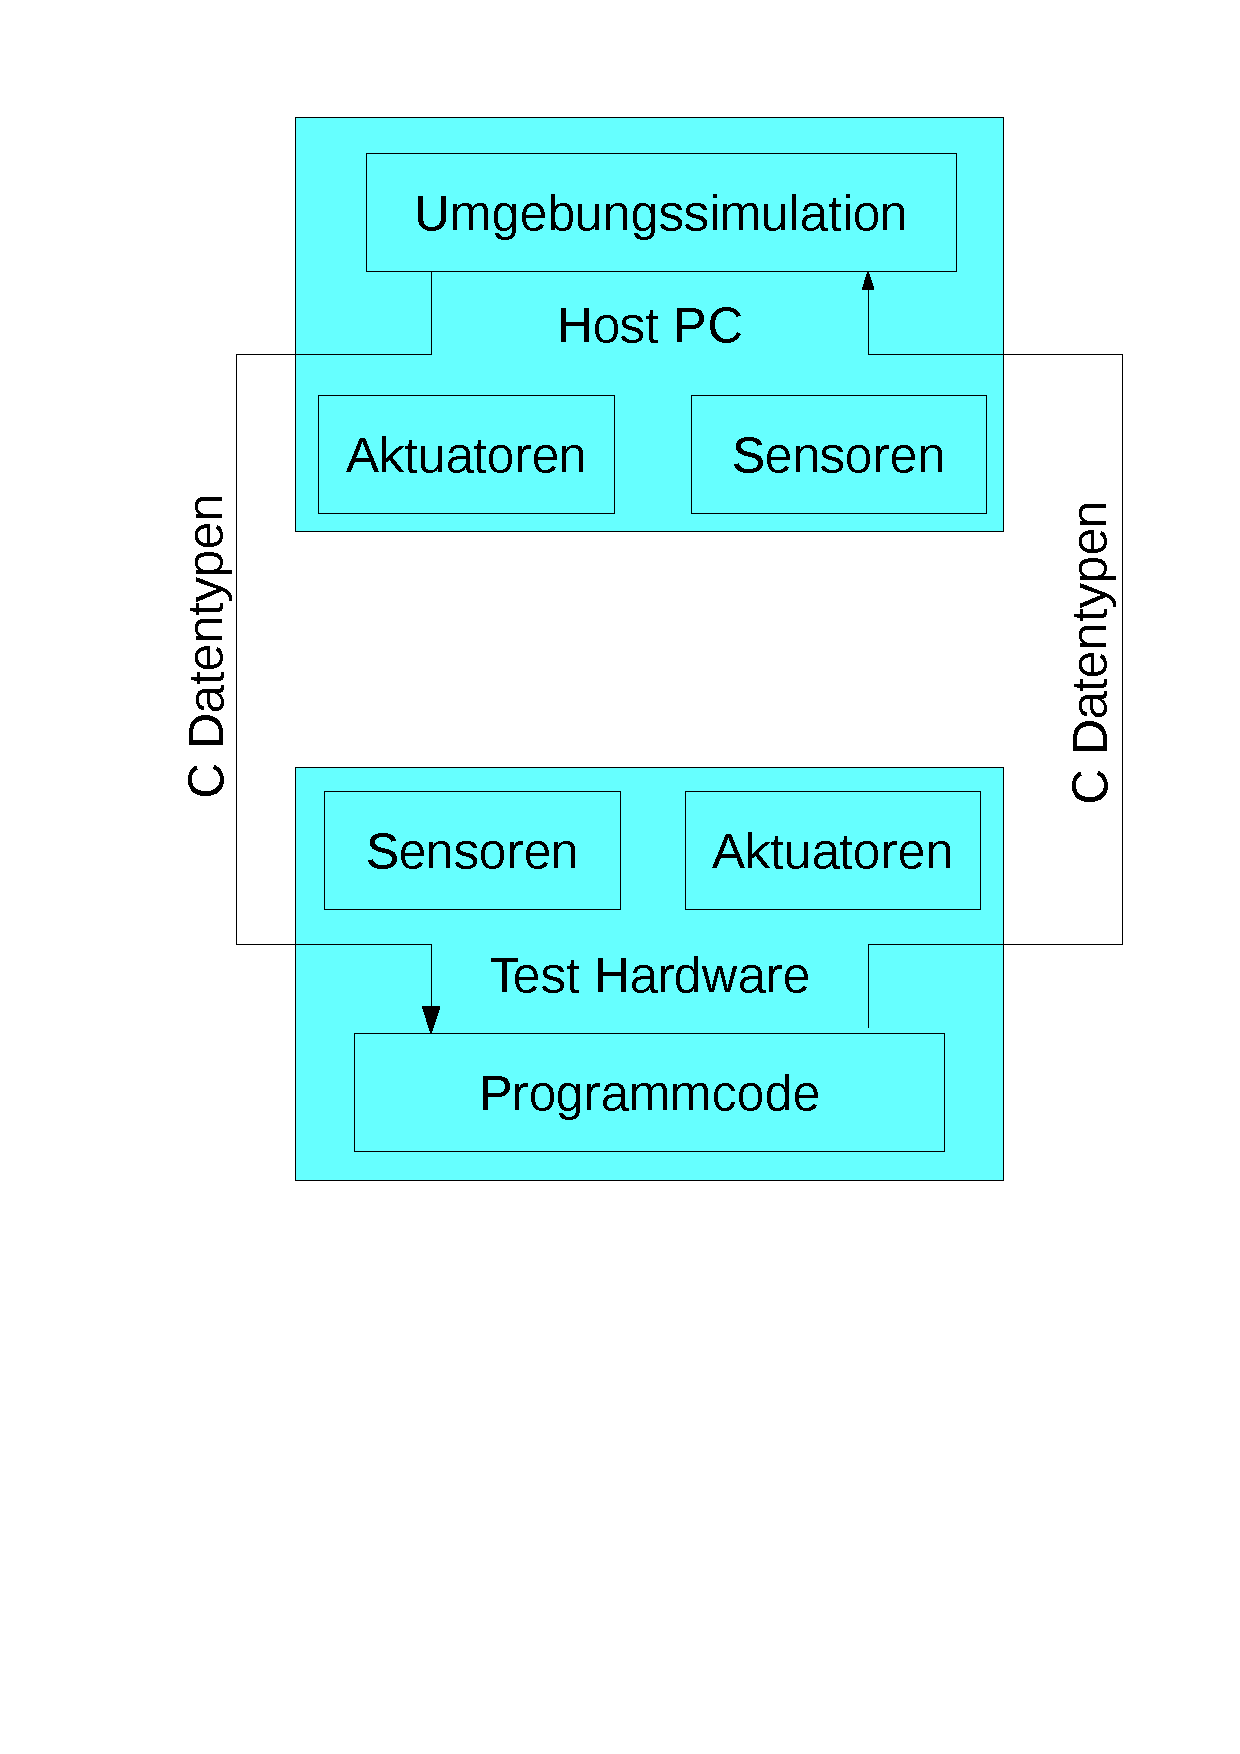
\includegraphics[height=0.33\paperheight, trim={3cm 9.5cm 1.5cm 2cm},clip]{pic/35_hil/hil_2.pdf}
		\caption{Pixhawk Hil Aufbau}
		\label{fig:hil_pixhawk}
		\end{center}
		\end{subfigure}
		\caption{Vergleich Hil Aufbau}
		\label{fig:hil_vergleich}
	\end{center}
\end{figure}

\noindent
Für die Pixhawk Simulation (Abbildung: \ref{fig:hil_pixhawk}) werden die elektrischen Signale abgegriffen, welche die Aktuatoren ansteuern würden. Dies senkt die Simulationskomplexität stark. Bei einer echten HiL Simulation (Abbildung: \ref{fig:hil_normal}) müssten die Aktuatoren und Sensoren der Test Hardware auch miteinbezogen werden.\\\\
Beispiel Rotoren:\\
Bei einer echten HiL Simulation würde der Rotorenschub der Test Hardware durch ein Anemometer gemessen. Dieses Signal würde dann in dem Umgebungssimulator ausgewertet und die Aktuatoren Stellgrössen berechnen.\\
Bei der Pixhawk HiL Simulation wird das PWM der Frequenzumrichter direkt an den Host PC per UART übermittelt. Die Aktautoren und Sensoren werden jeweils überbrückt.

\clearpage